\documentclass[../main.tex]{subfiles}
\graphicspath{{\subfix{../res/}}}
\begin{document}

As we embark on constructing our pipeline for data-driven student success prediction, we must first delineate the data inputs and algorithmic strategies. 
It is clear that by the results from our state of the art and analysis that a multifaceted algorithmic approach is warranted to optimize outcomes
To extract as much information and get the possible best results, we have split our system into three inner parts, each with their responsibility, input, and output.
But first, let's look into which data we have access to, and which we shall determine the pertinent data for ingestion into the system.

\subsection{Feeding data}
\label{subsec:conceptualimplementation_feedingdata}
Our literature survey has identified several key factors influencing student retention and success. We can extrapolate and hypothesis such wide factors could be used to determine student's success.
These factors, hypothesized to be critical in predicting student trajectories, are:

\begin{itemize}
    \item Family
    \item Previous educational background
    \item Academic potential
    \item Normative congruence
    \item Friendship support
    \item Intellectual development
    \item Educational performance
    \item Social integration
    \item Satisfaction
    \item Institutional commitment
    \item Student adaptation
    \item Strict School Rules
\end{itemize}

The available dataset for our experiment will be processed to align with these factors, ensuring that each is represented accurately to serve as a foundation for our predictive models.
\begin{itemize}
    \item Family
    \item Previous educational background
    \item Academic potential
    \item Normative congruence
    \item Friendship support
    \item Intellectual development
    \item Educational performance
    \item Social integration
    \item Satisfaction
    \item Institutional commitment
    \item Student adaptation
    \item Strict School Rules
\end{itemize}


\subsection{Data workflow}
\label{subsec:conceptualimplementation_dataworkflow}

Our workflow, as depicted in Figure \ref{fig:dataworkflow}, is designed to systematically transform raw data into actionable insights.

\begin{figure}
    \centering
    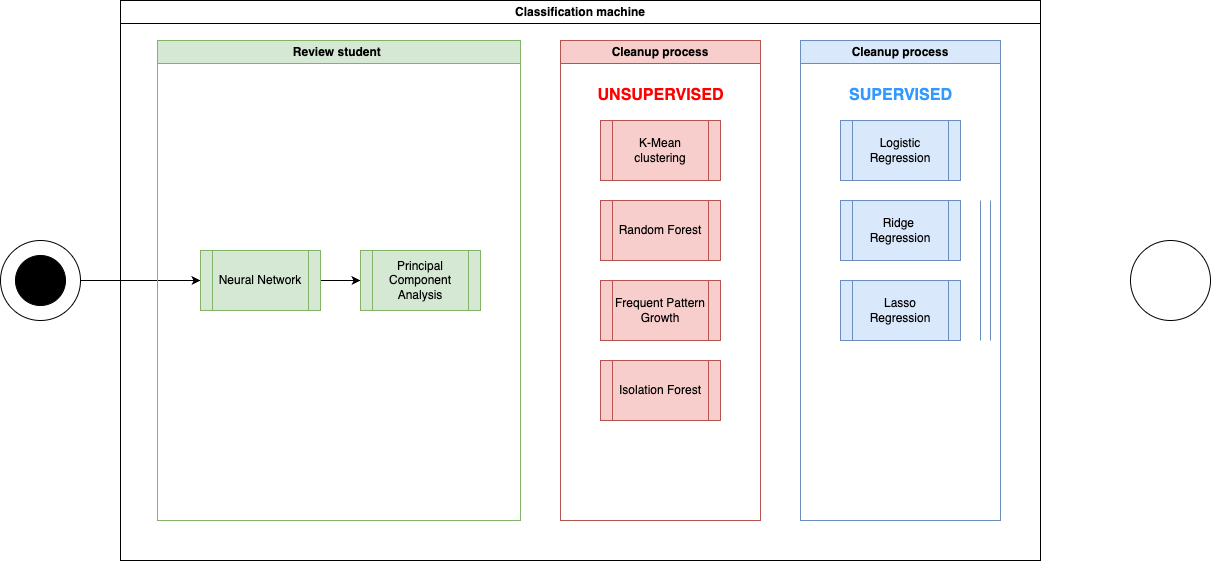
\includegraphics[width=1\linewidth]{res//diagram/ML Workflow.png}
    \caption{Algorithmic workflow for data-driven student success prediction.}
    \label{fig:dataworkflow}
\end{figure}

Each component of the workflow serves a strategic purpose:

\begin{enumerate}
    \item \acrfull{nn}: To model complex non-linear relationships and interactions among the input variables.
    \item \acrfull{pca}: For dimensionality reduction, facilitating computational efficiency and data visualization.
    \item K-Mean clustering: To identify natural groupings within the student population.
    \item Isolation Forest: For anomaly detection, highlighting atypical cases that may require special attention.
    \item Lasso Regression: To perform feature selection, enhancing model interoperability by isolating significant predictors.
\end{enumerate}

\subsection{Validation and Expected Outcomes}
The efficacy of our approach will be gauged through rigorous validation techniques, ensuring the reliability of our predictions. We anticipate that this comprehensive workflow will yield a robust predictive model capable of identifying students at risk and informing targeted interventions.

\end{document}